\section{TP1}
\subsection{M\'etricas, elementos de l\'inea y transformaciones de coordenadas}

Bajo una transformaci\'on de coordenadas a partir de coordenadas cartesianas (o inerciales) $\xi^{a} = \xi^{a}(x^{\mu})$, las m\'etricas euclidiana $\delta_{ab}$ o la de Minkowski $\eta_{ab}$ se transforman en una nueva
m\'etrica $g_{\mu \nu}$, de tal manera que las distancias propias son invariantes,

\begin{equation}
    (\delta_{ab}, \eta_{ab})d\xi^{a}d\xi^{b} = g_{\mu \nu}dx^{\mu}dx^{\nu} \iff g_{\mu \nu} = J_{\mu}^{a}J_{\nu}^{b}(\delta_{ab}, \eta_{ab})
    \label{eq1}
\end{equation}

con $J_{\mu}^{a} = \frac{\partial \xi^{a}}{\partial x^{\mu}}$, la matriz Jacobiana de la transformaci\'on.\\

\subsubsection{M\'etricas en 2D}

Considere el siguiente elemento de l\'inea bidimensional

\begin{equation}
    ds^{2} = (dy^{1})^{2} + (dy^{2})^{2} + 2ady^{1}dy^{2}
    \label{eq2}
\end{equation}

con $a \in \mathbb{R}$ constante.

\begin{itemize}
    \item Muestre que esta m\'etrica es no degenerada para $a \neq \pm 1$.
    \item Muestre que, para $a^{2} < 1$, la m\'etrica est\'a relacionada con la Euclideana $ds^{2} = (dx^{1})^{2} + (dx^{2})^{2}$ mediante la transformaci\'on.

    \begin{equation}
        x^{1} = \sqrt{1 - a^{2}}y^{1} \ , \ x^{2} = ay^{1} + y^{2}
        \label{eq3}
    \end{equation}

    \item Muestre que, para $a^{2} > 1$, la m\'etrica est\'a relacionada con la Lorentziana $ds^{2} = -dt^{2} + dx^{2}$ mediante alguna transformaci\'on.
\end{itemize}

\textbf{Soluci\'on:}\\

Es f\'acil ver que la m\'etrica adopta la siguiente forma matricial

$$g_{\mu \nu} =
    \begin{pmatrix}
    g_{y^{1}y^{1}} & g_{y^{1}y^{2}}\\
    g_{y^{2}y^{1}} & g_{y^{2}y^{2}}
    \end{pmatrix}
 = 
    \begin{pmatrix}
    1 & a\\
    a & 1
    \end{pmatrix}
$$\\

Luego, $g = \det(g_{\mu \nu}) = 1 - a^{2}$. Como $a \neq \pm 1$, entonces $g \neq 0$, por lo tanto la m\'etrica es no degenerada. $\checkmark$\\

Para $a^{2} > 1$, invertimos las transformaciones dadas (\ref{eq3}) en funci\'on de $y^{1}$ e $y^{2}$:

$$y^{1} = \frac{x^{1}}{\sqrt{1 - a^{2}}}$$

$$y^{2} = x^{2} - ay^{1} = x^{2} - a\frac{x^{1}}{\sqrt{1 - a^{2}}}$$

$$\Rightarrow dy^{1} = \frac{dx^{1}}{\sqrt{1 - a^{2}}} \ , \ dy^{2} = dx^{2} - a\frac{dx^{1}}{\sqrt{1 - a^{2}}}$$

Reemplazando esto en (\ref{eq2}), obtenemos

$$ds^{2} = \bigg(\frac{dx^{1}}{\sqrt{1 - a^{2}}}\bigg)^{2} + \bigg(dx^{2} - a\frac{dx^{1}}{\sqrt{1 - a^{2}}}\bigg)^{2} + 2a\bigg(\frac{dx^{1}}{\sqrt{1 - a^{2}}}\bigg)\bigg(dx^{2} - a\frac{dx^{1}}{\sqrt{1 - a^{2}}}\bigg)$$

$$ds^{2} = \frac{(dx^{1})^{2}}{1 - a^{2}} + (dx^{2})^{2} - 2a\frac{dx^{1}}{\sqrt{1 - a^{2}}}dx^{2} +  a^{2}\frac{(dx^{1})^{2}}{1 - a^{2}} + 2a\frac{dx^{1}}{\sqrt{1 - a^{2}}}dx^{2} - 2a^{2}\frac{(dx^{1})^{2}}{1 - a^{2}}$$

$$\Rightarrow ds^{2} = (1 - a^{2})\frac{(dx^{1})^{2}}{1 - a^{2}} + (dx^{2})^{2} = (dx^{1})^{2} + (dx^{2})^{2} \ \checkmark$$

Para $a^{2} < 1$, se proponen las siguientes transformaciones:

$$t = \sqrt{a^{2} - 1}y^{1} \Rightarrow dt = \sqrt{a^{2} - 1}dy^{1}$$

$$x = ay^{1} + y^{2} \Rightarrow dx = ady^{1} + dy^{2}$$

Haciendo el mismo c\'alculo que en el punto anterior, obtenemos

$$ds^{2} = -dt^{2} + dx^{2}$$

\subsubsection{M\'etrica de Rindler}

Considere la m\'etrica de Minkowski (1+1)-dimensional con elemento de l\'inea $ds^{2} = -dt^{2} + dx^{2}$, y las \textit{coordenadas de Rindler} $(T, X)$ definidas como

\begin{equation}
    t = X\sinh{T} \ , \ x = X\cosh{T}
    \label{eq4}
\end{equation}

con $a \in \mathbb{R}$ constante.

\begin{itemize}
    \item Determine la m\'etrica o elemento de l\'inea en estas coordenadas.
    \item Muestre que las l\'ineas $T = cte$, $X = cte$ son l\'ineas rectas que pasan por el origen o hiperbolas (en un diagrama $(t, x)$), respectivamente.
\end{itemize}

\textbf{Soluci\'on:}\\

Diferenciando las nuevas coordenadas

$$dt = dX\sinh{T} + X\cosh{T}dT$$

$$dx = dX\cosh{T} + X\sinh{T}dT$$\\

Elevando al cuadrado ambas igualdades

$$dt^{2} = (dX\sinh{T} + X\cosh{T}dT)^{2} = dX^{2}\sinh^{2}{T} + 2XdX\sinh{T}\cosh{T}dT + X^{2}\cosh^{2}{T}dT^{2}$$

$$dx^{2} = (dX\cosh{T} + X\sinh{T}dT)^{2} = dX^{2}\cosh^{2}{T} + 2XdX\cosh{T}\sinh{T}dT + X^{2}\sinh^{2}{T}dT^{2}$$\\

Reemplaz\'andolas en $ds^{2} = -dt^{2} + dx^{2}$:

$$ds^{2} = -dX^{2}\sinh^{2}{T} - 2XdX\sinh{T}\cosh{T}dT - X^{2}\cosh^{2}{T}dT^{2}$$
$$+ dX^{2}\cosh^{2}{T} + 2XdX\cosh{T}\sinh{T}dT + X^{2}\sinh^{2}{T}dT^{2}$$\\
$$\Rightarrow ds^{2} = (dX^{2} - X^{2}dT^{2})(\cosh^{2}{T} - \sinh^{2}{T}) =  - X^{2}dT^{2} + dX^{2} \ \checkmark$$\\

Para $T = T_{0}$ constante, las ecuaciones (\ref{eq4}) nos quedan:

$$t = X\sinh{T_{0}} \ , \ x = X\cosh{T_{0}}$$

$$\Rightarrow t = \frac{x}{\cosh{T_{0}}}\sinh{T_{0}} = x\tanh{T_{0}}\  \checkmark$$

es la ecuaci\'on de una recta que pasa por el origen.\\

Tomando $X = X_{0}$ constante, obtenemos de las ecuaciones (\ref{eq4}):

$$t = X_{0}\sinh{T} \ , \ x = X_{0}\cosh{T}$$

$$\Rightarrow t^{2} = X_{0}^{2}\sinh^{2}{T} \ , \ x^{2} = X_{0}^{2}\cosh^{2}{T}$$

Restando ambos cuadrados

$$t^{2} - x^{2} = X_{0}^{2}(\sinh^{2}{T} - \cosh^{2}{T}) = X_{0}^{2}\ \checkmark$$

describiendo una hip\'erbola en el plano $(t, x)$.

\begin{figure}[H]
    \centering
    \begin{subfigure}[b]{0.5\linewidth}
        \fbox{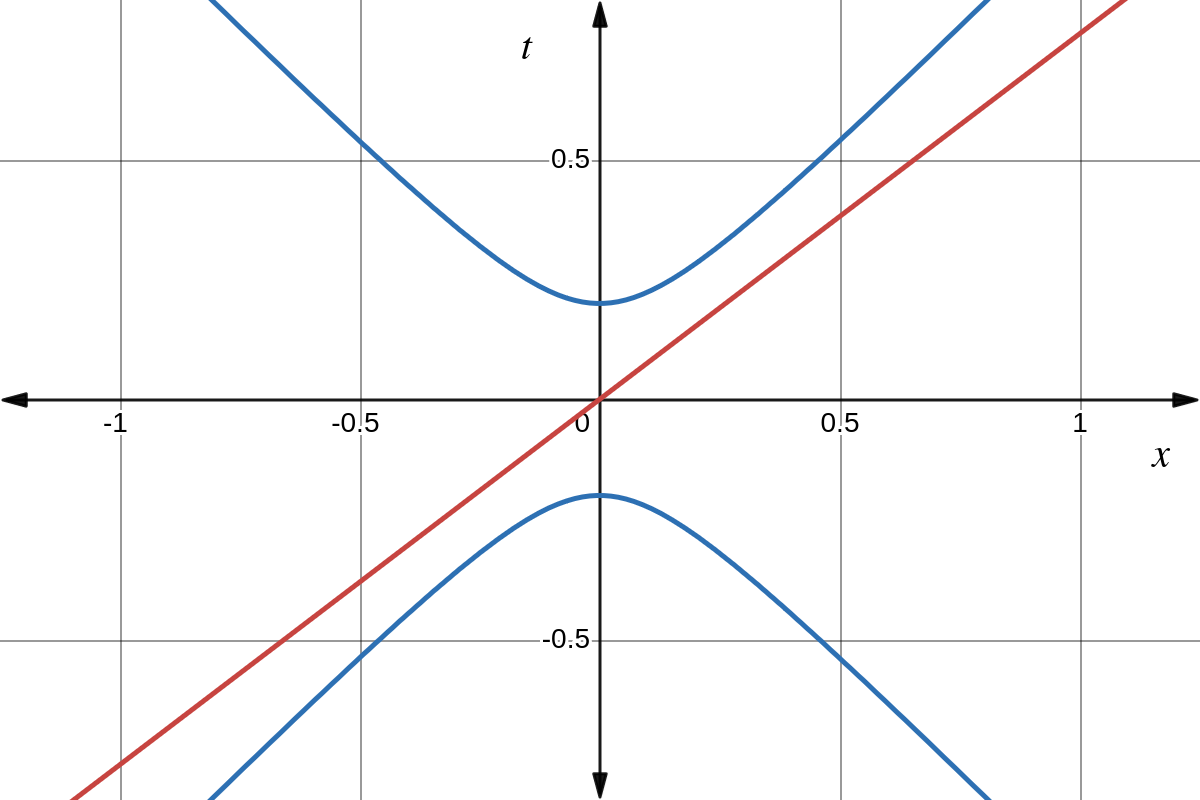
\includegraphics[width=\linewidth]{A1/a1_ex1.png}}
    \end{subfigure}
    \caption{Recta $t = x\tanh{T_{0}}$ (rojo) e hip\'erbola $t^{2} - x^{2} = X_{0}^{2}$ (azul), con constantes $T_{0} = 1$ y $X_{0} = 0.2$, respectivamente.}
    \label{fig:cap1_trappedsurface}
\end{figure}

\subsection{Geod\'esicas I}

\subsubsection{Geod\'esicas y ecuaciones de Euler-Lagrange}

Muestre que las ecuaciones de Euler-Lagrange

\begin{equation}
    \frac{d}{d\lambda}\frac{\partial \mathcal{L}}{\partial x'^{\mu}} - \frac{\partial \mathcal{L}}{\partial x^{\mu}} = 0
    \label{eq5}
\end{equation}

para el Lagrangiano

\begin{equation}
    \mathcal{L} = \frac{1}{2}g_{\mu \nu}\frac{dx^{\mu}}{d\lambda}\frac{dx^{\nu}}{d\lambda} = \frac{1}{2}g_{\mu \nu}x'^{\mu}x'^{\nu}
    \label{eq6}
\end{equation}

son las ecuaciones geod\'esicas

\begin{equation}
    \frac{d^{2}x^{\mu}}{d\lambda^{2}} + \Gamma^{\mu}_{\nu \lambda}\frac{dx^{\nu}}{d\lambda}\frac{dx^{\lambda}}{d\lambda} = 0
    \label{eq7}
\end{equation}

donde los \textit{s\'imbolos de Christoffel} $\Gamma^{\mu}_{\nu \lambda}$ asociados a la m\'etrica $g_{\mu \nu}$ se definen como

\begin{equation}
    \Gamma^{\mu}_{\nu \lambda} = g^{\mu \rho}\Gamma_{\rho \nu \lambda} = \frac{1}{2}g^{\mu \rho}(\partial_{\lambda}g_{\nu \rho} + \partial_{\nu}g_{\rho \lambda} - \partial_{\rho}g_{\nu \lambda})
    \label{eq8}
\end{equation}\\

\textbf{Soluci\'on:}\\

Calculemos el primer t\'ermino de la ecuaci\'on (\ref{eq5}) usando (\ref{eq6}):

$$\frac{d}{d\tau}\bigg(\frac{\partial \mathcal{L}}{\partial x'^{\gamma}}\bigg) = \frac{d}{d\tau}\bigg(g_{\gamma \nu}x'^{\nu}\bigg)$$

El segundo t\'ermino queda de la siguiente manera:

$$\frac{\partial \mathcal{L}}{\partial x^{\gamma}} = \frac{1}{2}\partial_{\gamma}g_{\mu \nu}x'^{\mu}x'^{\nu}$$\\

Juntando todo en (\ref{eq5})

$$\frac{d}{d\tau}(g_{\gamma \nu}x'^{\nu}) - \frac{1}{2}\partial_{\gamma}g_{\mu \nu}x'^{\mu}x'^{\nu} = \frac{d}{d\tau}(g_{\gamma \nu})x'^{\nu} + g_{\gamma \nu}\frac{d}{d\tau}(x'^{\nu}) - \frac{1}{2}\partial_{\gamma}g_{\mu \nu}x'^{\mu}x'^{\nu}$$\\

Veamos por separado los dos primeros t\'erminos del lado derecho de esta \'ultima igualdad:

$$\frac{d}{d\tau}(g_{\gamma \nu})x'^{\nu} = \partial_{\mu}g_{\gamma \nu}x'^{\mu}x'^{\nu}$$

$$g_{\gamma \nu}\frac{d}{d\tau}(x'^{\nu}) = g_{\gamma \nu}x''^{\nu}$$\\

Luego

$$\partial_{\mu}g_{\gamma \nu}x'^{\mu}x'^{\nu} + g_{\gamma \nu}x''^{\nu} - \frac{1}{2}\partial_{\gamma}g_{\mu \nu}x'^{\mu}x'^{\nu} = 0$$

$$\Rightarrow  \frac{1}{2}(\partial_{\mu} g_{\gamma \nu} + \partial_{\nu} g_{\gamma \beta})x'^{\mu}x'^{\nu} + g_{\gamma \nu}x''^{\nu} - \frac{1}{2}\partial_{\gamma}g_{\mu \nu}x'^{\mu}x'^{\nu} = 0$$\\

(el primer t\'ermino se puede escribir as\'i porque $x'^{\mu}x'^{\nu} = x'^{\nu}x'^{\mu}$ es sim\'etrico). Reagrupando el primero y \'ultimo del lado izquierdo:

$$g_{\gamma \nu}x''^{\nu} + \frac{1}{2}(\partial_{\mu} g_{\gamma \nu} + \partial_{\nu} g_{\gamma \beta} - \partial_{\gamma}g_{\mu \nu})x'^{\mu}x'^{\nu} = 0$$\\

El segundo t\'ermino es el \textit{s\'imbolo de Christoffel de primer tipo} $\Gamma_{\gamma \mu \nu}$, por lo tanto

$$g_{\gamma \nu}x''^{\nu} + \Gamma_{\gamma \mu \nu}x'^{\mu}x'^{\nu} = 0$$\\

Si multiplicamos por $g^{\gamma \rho}$ (m\'etrica inversa) para elevar uno de los \'indices, obtenemos finalmente (\ref{eq7}):

$$g^{\gamma \rho}g_{\rho \nu}x''^{\nu} + g^{\gamma \rho}\Gamma_{\rho \mu \nu}x'^{\mu}x'^{\nu} = 0$$\\

$$\Rightarrow x''^{\gamma} + \Gamma^{\gamma}_{\mu \nu}x'^{\mu}x'^{\nu} = 0 \ \checkmark$$\\

\subsubsection{$\mathcal{L}$ es una constante de movimiento}

Muestre que $\mathcal{L}$ es constante a lo largo de cualquier geod\'esica, es decir

\begin{equation}
    \frac{d}{d\lambda}\bigg( g^{\mu \nu}\frac{dx^{\mu}}{d\lambda}\frac{dx^{\nu}}{d\lambda} \bigg) = 0
    \label{eq9}
\end{equation}

para $x^{\mu}(\lambda)$ soluci\'on de la ecuaci\'on geod\'esica.

¿Cual es la simetr\'ia, por el teorema de Noether, que da lugar a esta constante de movimiento?\\

\textbf{Soluci\'on:}\\

Es bastante autom\'atico si procedemos como en el punto anterior. Nuevamente

$$\frac{d}{d\tau}(g_{\mu \nu}) = \partial_{\gamma}g_{\mu \nu}x'^{\gamma}$$

$$\Rightarrow \frac{d\mathcal{L}}{d\tau} = \partial_{\gamma}g_{\mu \nu}x'^{\mu}x'^{\nu}x'^{\gamma} + 2g_{\mu \nu}x''^{\mu}x'^{\nu}$$\\

Usando la identidad $\partial_{\gamma}g_{\mu \nu} = \Gamma_{\mu \nu \gamma} + \Gamma_{\nu \mu \gamma}$, entonces $\partial_{\gamma}g_{\mu\nu}x'^{\mu}x'^{\nu}x'^{\gamma} = 2\Gamma_{\nu \mu \gamma}x'^{\mu}x'^{\nu}x'^{\gamma}$. Por lo tanto

$$\frac{d\mathcal{L}}{d\tau} = 2(g_{\nu \mu}x''^{\mu} + \Gamma_{\nu \mu \gamma}x'^{\mu}x'^{\gamma})x'^{\nu}$$

la cual se anula por ser una soluci\'on de la geod\'esica.\\

La simetr\'ia que corresponde a esta cantidad conservada es la traslaci\'on en $\tau$ (dado que el Lagrangiano no depende expl\'icitamente de este par\'ametro, la energ\'ia correspondiente se conserva).